

\documentclass{beamer}
\usetheme{Berkeley}			%Berkeley Goettingen Hannover Berlin
\usecolortheme{seagull} 	%beaver dolphin
\usepackage{german}



\begin{document}

\title{\textcolor{black}{Python-Projekt: Sudoku Solver}}   
\author{Leander Teichmann, Florian Herrmann} 
\date{\today}
\logo{
\includegraphics[scale=0.3]{img/HAWK_Logo.jpg}}

\begin{frame}
\titlepage
\end{frame}


\begin{frame}
\frametitle{Inhaltsverzeichnis}\tableofcontents
\end{frame}

\section{Was ist ein Sudoku?}
\begin{frame}
	\frametitle{Was ist ein Sudoku?} 
	\begin{minipage}{0.48\textwidth}
	\begin{itemize}
		\item Das Spielfeld besteht aus $9 \cdot 9$ Feldern
		\item In der Regel: $n = 9$
		\item Ziel: Alle leeren Felder mit Zahlen füllen, sodass die Zahlen von 1 - 9 jeweils nur einmal vorkommen 
		\item in jeder Spalte 
		\item in jeder Reihe 
		\item in jedem der neun kleineren Quadrate
	\end{itemize} 
	\end{minipage}
	\begin{minipage}{0.48\textwidth}
		\centering
		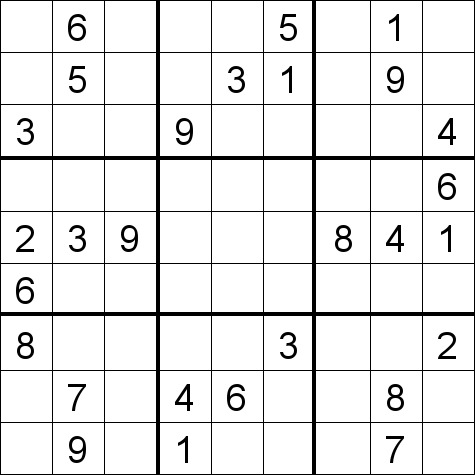
\includegraphics[width=0.95\textwidth]{img/sudoku.jpg}
	\end{minipage}
\end{frame}

\section{Projektaufbau:}
\begin{frame}
	\frametitle{Projektaufbau:} 
	\textbf{Ziele:}\\
	\textbf{Muss}:\\
	 Sudoku-Solver\\
	\textbf{Soll:} \\
	Dokumentation\\
	Variable Sudoku-Gittergröße\\
	\textbf{Kann:} \\
	GUI\\
	Versionsverwaltung mit git\\
	Organisation mit Agantty (Gantt-chart)
\end{frame}

\section{Was ist Rekursion?}
\begin{frame}
	\frametitle{Was ist Rekursion?} 
	\begin{minipage}{0.48\textwidth}
		Rekursion ist ein Programmierkonzept, bei der eine Funktion nur einen kleinen Teil des Problems löst und damit ein Problem ein bisschen verkleinter, und sich dann selbst aufruft um den Rest des Problems zu lösen.\\
		Das wird so lange fortgesetzt, bis das Problem gelöst ist.
	\end{minipage}
	\begin{minipage}{0.48\textwidth}
	\centering
	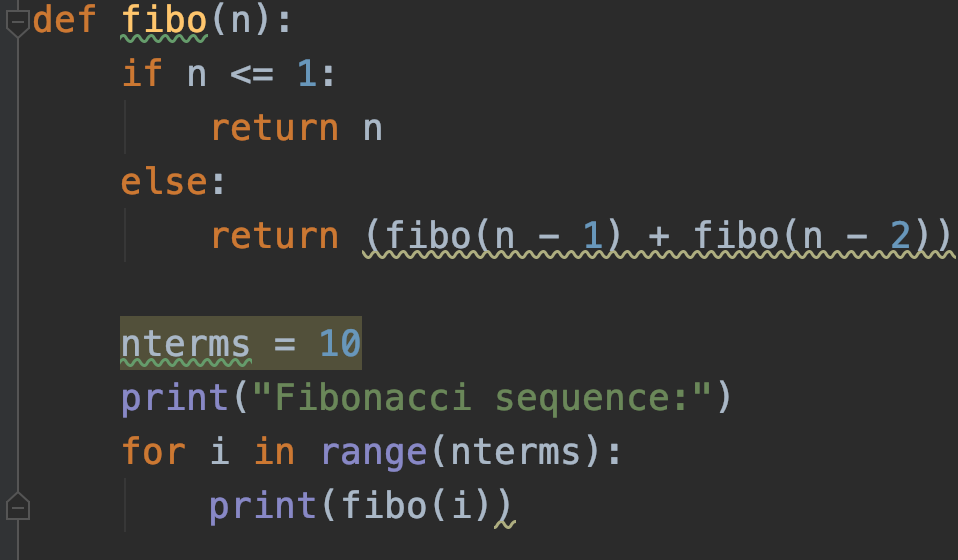
\includegraphics[width=0.95\textwidth]{img/fibo.png}
	\flushleft
	Fibonacci sequence:\\
	0\\
	1\\
	1\\
	2\\
	3\\
	5\\
	8\\
	13\\
	\end{minipage}
\end{frame}

\section{Lösungsstrategie}
\begin{frame}
	\frametitle{Lösungstrategie} 
	\begin{itemize}
		\item Backtracking (deutsch: Rücksetzverfahren) bezeichnet eine Problemlösungsmethode innerhalb der Algorithmik. 
		\item Trial-and-Error-Prinzip
	\end{itemize}
\end{frame}

\begin{frame}
	\frametitle{Lösungstrategie} 

	\textbf{Backtracking beim Susokulösen:}
	
	\begin{itemize}
		\item [1.] Suchen eines leeres Feldes
\item [2.] Versuchen, die Ziffern 1 - 9 an dieser Stelle zu platzieren
	\item [3.] Prüfen anhand des aktuellen Gitters, ob diese Ziffer an der aktuellen Stelle gültig ist
	\item [a.] Wenn die Ziffer gültig ist: Versuchen das Gitter rekursiv mit den Schritten 1 - 3 zu füllen.
	\item [b.] Wenn sie nicht gültig ist: Setzen des gerade gefüllten Feld auf 0 und zurückgehen zum vorherigen Schritt.
	\end{itemize}
	\textbf{Ist das Gitter voll, wurde eine Lösung gefunden.}
\end{frame}

\begin{frame}
	\frametitle{Lösungstrategie} 
	Flowchart des Lösungsalgorithmuses:
		\centering
	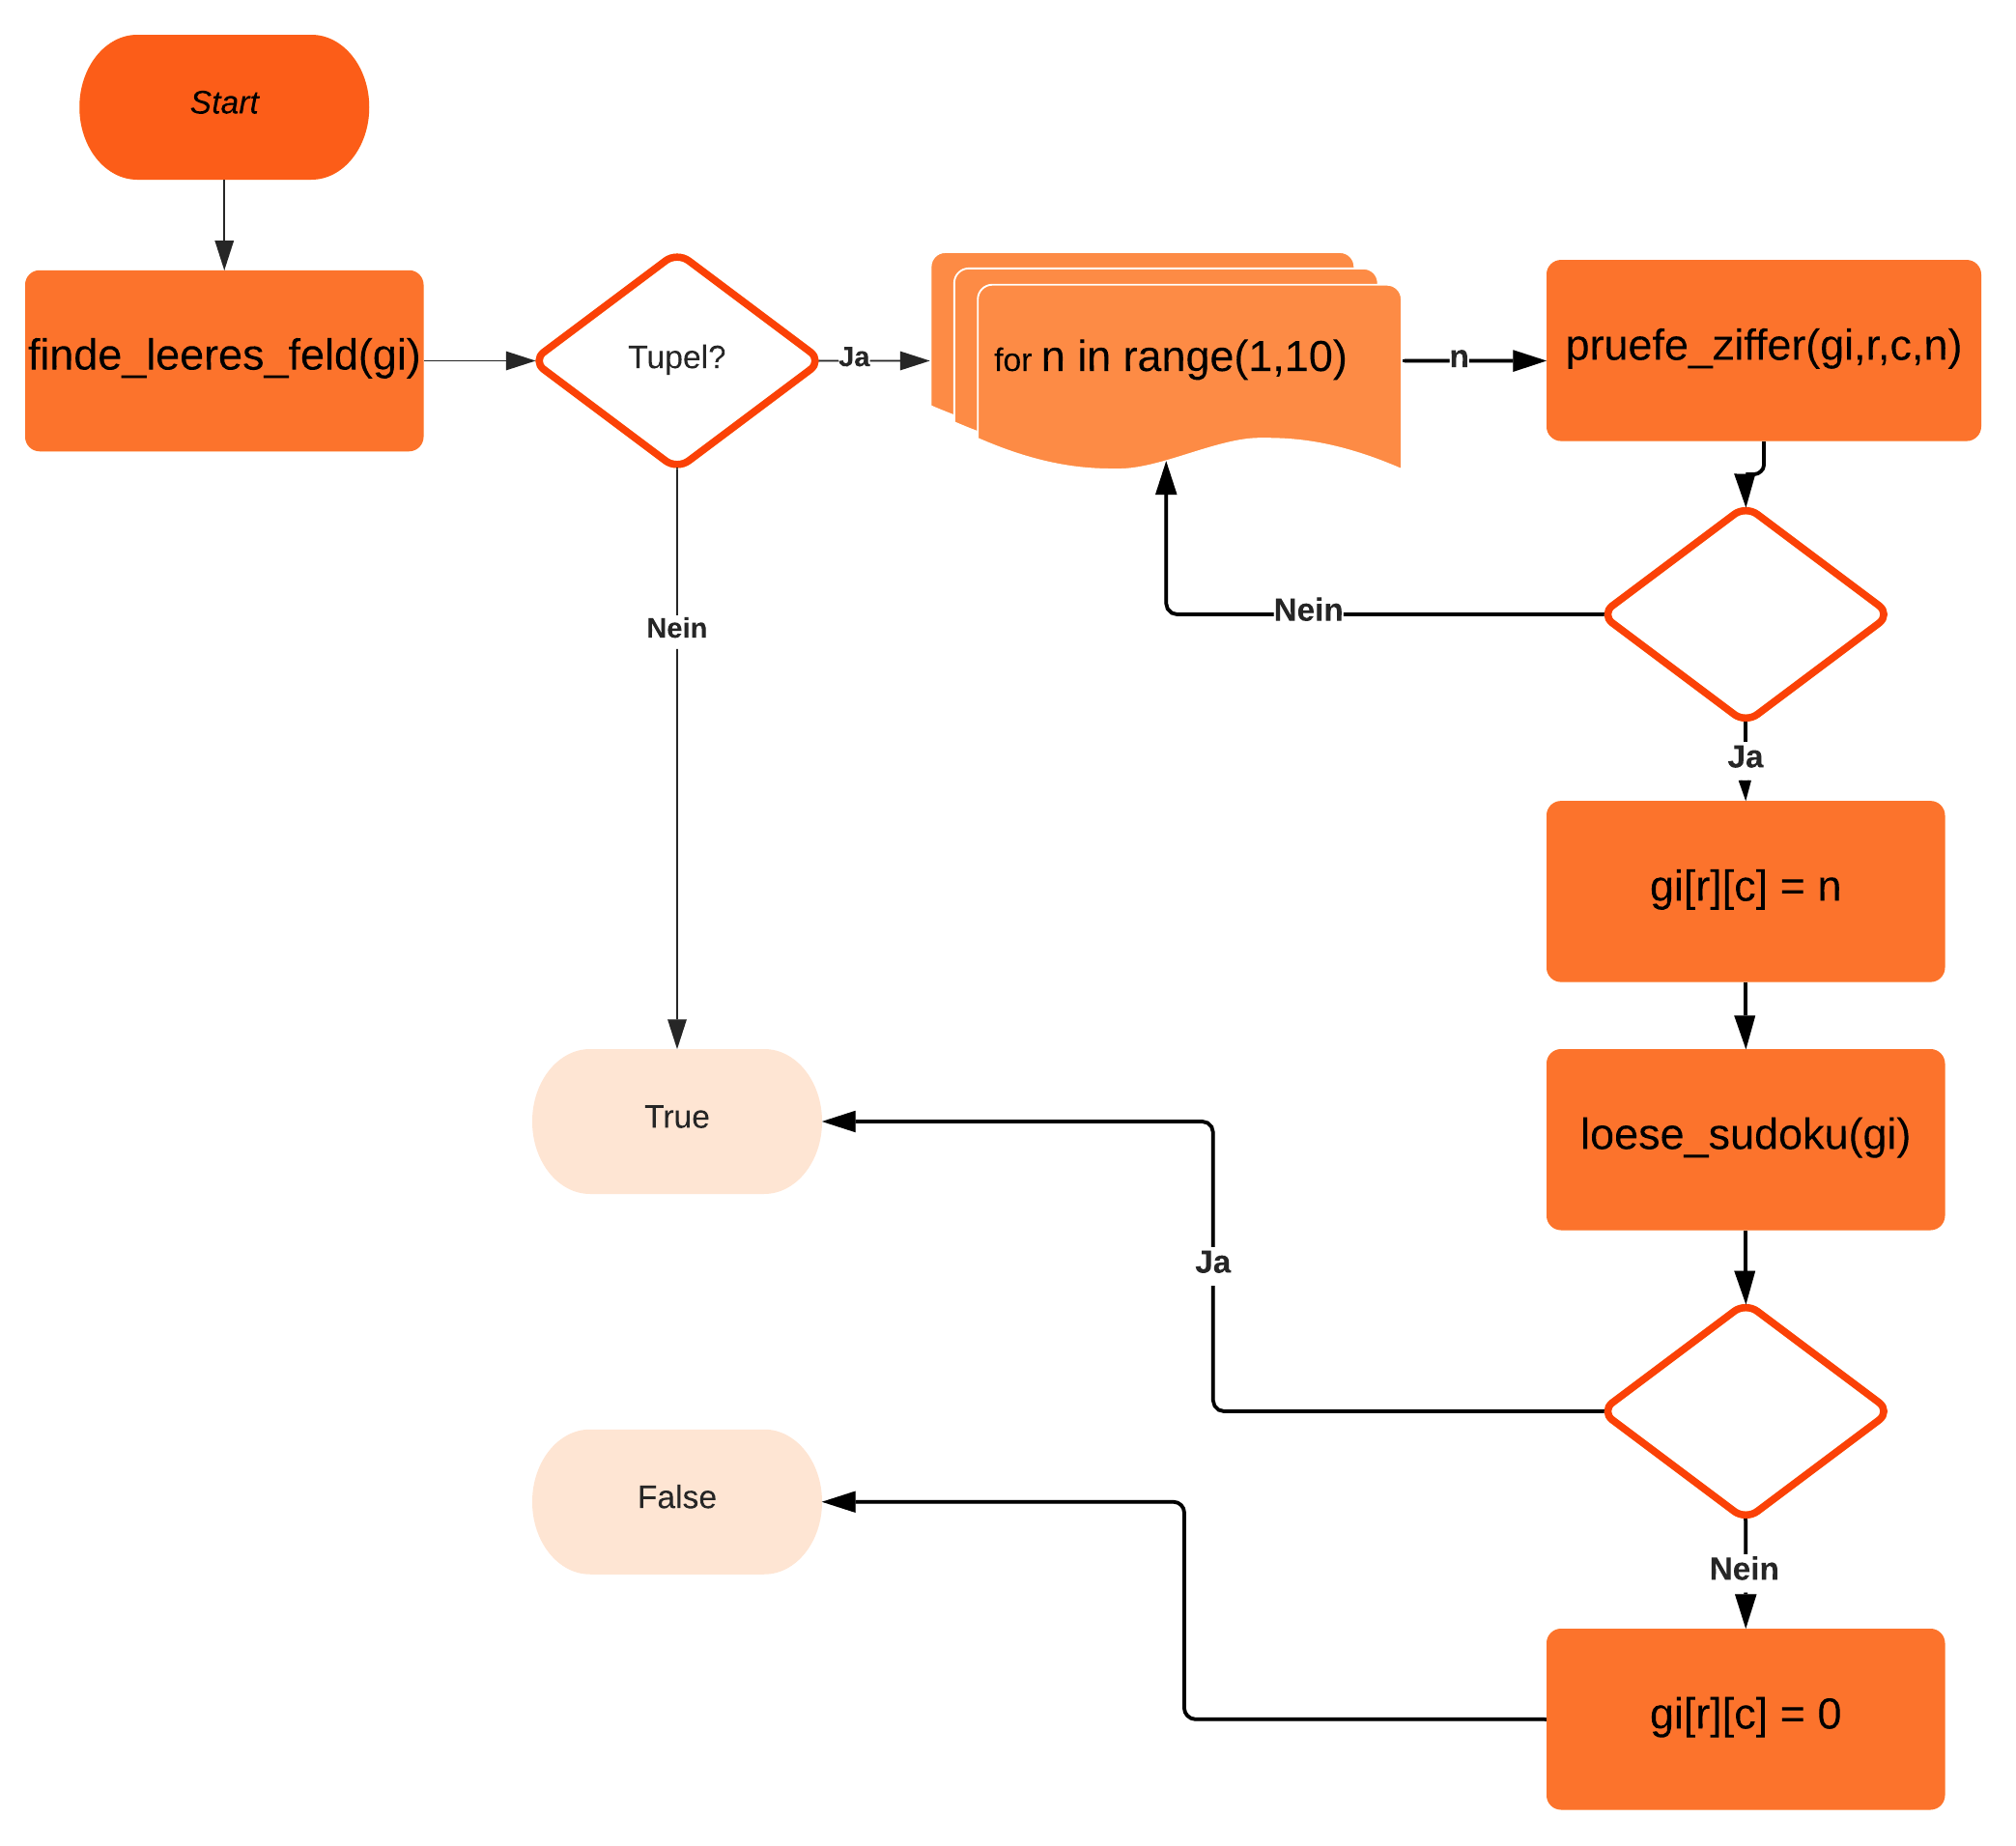
\includegraphics[width=0.95\textwidth]{img/flow.png}
\end{frame}

\section{GUI}
\begin{frame}
	\frametitle{GUI} 

	\textbf{GUI mit Pygame}\\
	Spielfeld besteht aus verschieden Instanzen von Klassen:\\
	\begin{minipage}{0.48\textwidth}
	\textbf{Felder}
	\begin{itemize}
		\item X Position
		\item Y Position
		\item Inhalt des Feldes
	\end{itemize}
	\textbf{Button}
	\begin{itemize}
		\item X Position
		\item Y Position
		\item Breite
		\item Höhe
		\item Beschriftung
	\end{itemize}

\end{minipage}
\begin{minipage}{0.48\textwidth}
	\textbf{Funktionen von Felder}
	\begin{itemize}
		\item Init
		\item Draw
		\item Select
	\end{itemize}

\textbf{Funktionen von Button}
\begin{itemize}
	\item Init
	\item Draw
	\item Select
\end{itemize}
\end{minipage}
\end{frame}

\begin{frame}
	\frametitle{GUI Ergebnis:} 
	Fertiges GUI:\\
	\centering
	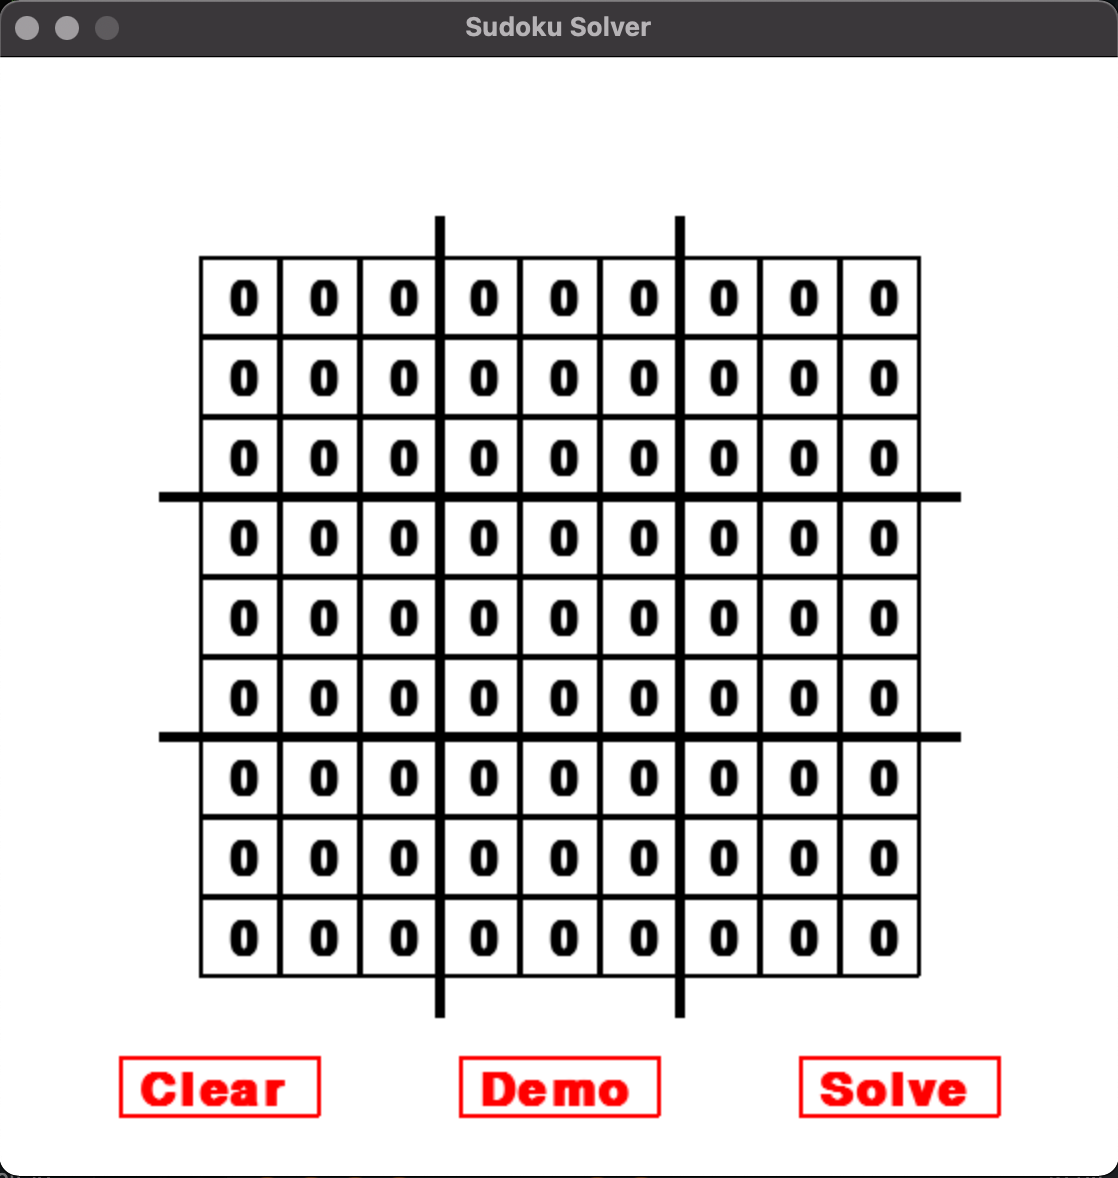
\includegraphics[width=0.6\textwidth]{img/gui.png}
\end{frame}

\section{Fazit}
\begin{frame}
	\frametitle{Fazit} 
	\textbf{Muss:} \\
	Sudoku-Solver $\Rightarrow$ Mittels Backtracking\\
	\textbf{Soll:}\
		Dokumentation $\Rightarrow$ Docstrings\\
		Variable Sudoku-Gittergröße $\Rightarrow$ In der Library implementiert\\
		Ab 16x16 großer Rechenaufwand. In der Komplexität reduzierte 16x16-Gitter\\ können in kurzer Zeit gelöst werden.\\
		\textbf{Kann: }\\
		GUI $\Rightarrow$ Mittels Pygame\\
		
		\textbf{Learnings:}\\
		Konzepte Rekursion und Backtracking\\
		Pygame\\
		Verbesserung von Projektorganisationsstrukturen\\
		Kennenlernen von git\\
	\end{frame}

\end{document}
